\documentclass{beamer}
\usepackage{graphicx}
\usepackage[utf8]{inputenc} %pour les accents
\usepackage[T1]{fontenc} %pour les accents
\usepackage{amsmath}
\usepackage{amsfonts}
\usepackage{amssymb}
\usepackage{stmaryrd}
\usepackage{makeidx}
\usepackage{amsthm}
\usepackage{mathrsfs}
\usepackage[francais]{babel}
\usepackage{eurosym}
\usepackage{tikz}

\usepackage{xcolor}
\usepackage{listings}

\usetikzlibrary{backgrounds,calc,shadings,shapes.arrows,shapes.symbols,shadows}
\tikzset{every picture/.style={execute at begin picture={
   \shorthandoff{:;!?};}
}}

\input{setTikz.tex}

\definecolor{dkgreen}{rgb}{0,0.6,0}
\definecolor{gray}{rgb}{0.5,0.5,0.5}
\definecolor{mauve}{rgb}{0.58,0,0.82}
\definecolor{redW}{rgb}{1,0.5,0.3}

\lstset{frame=tb,
  aboveskip=1mm,
  belowskip=1mm,
  showstringspaces=false,
  columns=flexible,
  basicstyle={\footnotesize\ttfamily},
  numbers=none,
  numberstyle=\tiny\color{gray},
  keywordstyle=\color{blue},
  commentstyle=\color{dkgreen},
  stringstyle=\color{mauve},
  breaklines=true,
  breakatwhitespace=true,
  tabsize=2
}

\lstdefinelanguage{plm}
{
keywordstyle=[2]
morekeywords={interface, Vlan, line, ip, hostname, no},
sensitive=false,
morecomment=[l]{!},
morecomment=[s]{/*}{*/},
%morestring=[b]",
%classoffset=0,
%morekeywords={standby},keywordstyle=\color{redW},
classoffset=1,
morekeywords={os, plm_version, evt_type, java_version, start_date, course, exolang, exoswitchto, totaltests, passedtests, exoname},keywordstyle=\color{blue},
classoffset=0
}

\usetheme{Luebeck}
\useoutertheme{split}
\useinnertheme{rectangles}
\usecolortheme{whale}
\usecolortheme{orchid}
\setbeamertemplate{navigation symbols}{\insertframenumber/\inserttotalframenumber}
\title[Serveur d’application pour la PLM]{Serveur d’application pour la Programmer’s Learning Machine}
\subtitle{Mathieu Morainville \& Cédric Huguenin}
\institute{Encadrants : Martin Quinson \& Gérald Oster \\ TELECOM Nancy}
\titlegraphic{\includegraphics[width=2.5cm,height=2.5cm,keepaspectratio]{images/TN}
$\quad$ \includegraphics[width=2.5cm,height=2.5cm,keepaspectratio]{images/loria}
} 
\begin{document}
 \begin{frame}
  \titlepage
 \end{frame}
 \begin{frame}
 	\frametitle{Introduction} % Introduction
 	La PLM permet :
 	\begin{itemize}
 	\item d'initier les étudiants venant des CPGE à la programmation ;
 	\item de faire des exercices d'algorithmiques plus avancés ;
 	\item de simplement apprendre à programmer.
 	\end{itemize}
 	\begin{center}
 	\onslide 
\includegraphics[scale=0.1]{images/buggle.eps}
 	\end{center}
 \end{frame}
  \begin{frame}
  \tableofcontents
 \end{frame}
\section{Problématiques}
	\begin{frame}
		\tableofcontents[currentsection]
	\end{frame}
	\begin{frame}
	\frametitle{Problèmes actuels}
		\begin{itemize}
		\item beaucoup d'élèves dans des salles différentes ;
		\item certains travaillent à la maison ;
		\item suivi difficile ;
		\item PLM pas optimisée pour un usage sur plusieurs machines ;
		\item pas de suivi du code ;
		\item un seul utilisateur par machine.
		\end{itemize}
	\end{frame}

\section{Solutions}
	\begin{frame}
	\tableofcontents[currentsection]
\end{frame}
\begin{frame}
	\frametitle{GitSession \& GitSpy}
	\begin{itemize}
		\item Dépôt git local ;
		\item un dépôt par utilisateur.
	\end{itemize}
	\begin{center}
		\begin{tikzpicture}
			\node[server](PC1) at (-3,0) {};
			\node[xshift=-0.8cm,yshift=0.2cm,left of = PC1,align=left](PC1label) {Utilisateurs A};
			
			\node(GitA1) at (-5.5,-2) {\includegraphics[scale=0.25]{images/git.ps}}; 
			\node[below of = GitA1,align=left](GitAlabel1) {Git local utilisateur A1};
			
			\node(GitA2) at (-0.5,-2) {\includegraphics[scale=0.25]{images/git.ps}}; 
			\node[below of = GitA2,align=left](GitAlabel1) {Git local utilisateur A2};
			
			\draw[thick,darkgray!10!gray] (PC1.south east)--(GitA1);
			\draw[thick,darkgray!10!gray] (PC1.south west)--(GitA2);
		\end{tikzpicture}
	\end{center}
\end{frame}
\begin{frame}[containsverbatim]
	\frametitle{Exemples de commit}
	\begin{itemize}
		\item Type de l'évènement, exercice, nombre de tests passés / total, etc.
	\end{itemize}
		\begin{lstlisting}[language = plm,basicstyle={\scriptsize\ttfamily}, caption= Message de commit]
{"os":"Windows 8 (version: 6.2; arch: amd64)","plm_version":"2.3beta (20140125)","evt_type":"started","java_version":"1.7.0_51 (VM: Java HotSpot(TM) 64-Bit Server VM; version: 24.51-b03)","start_date":"2014\/05\/21 13:08:26"}

{"course":"","exolang":"Java","evt_type":"executed","totaltests":"1", "passedtests":"1","exoname":"Welcome in the Buggles' World"}
		\end{lstlisting}
\end{frame}


\begin{frame}
	\frametitle{Serveur distant}
	\begin{itemize}
	\item Git distant qui centralise les données :
	\end{itemize}
	\begin{center}
		\input{gitDistant.tex}
	\end{center}
\end{frame}

\begin{frame}
	\frametitle{Serveur distant}
	\begin{itemize}
	\item Une branche par utilisateur identifié par le hash d'un numéro unique :
	\end{itemize}
	\begin{center}
		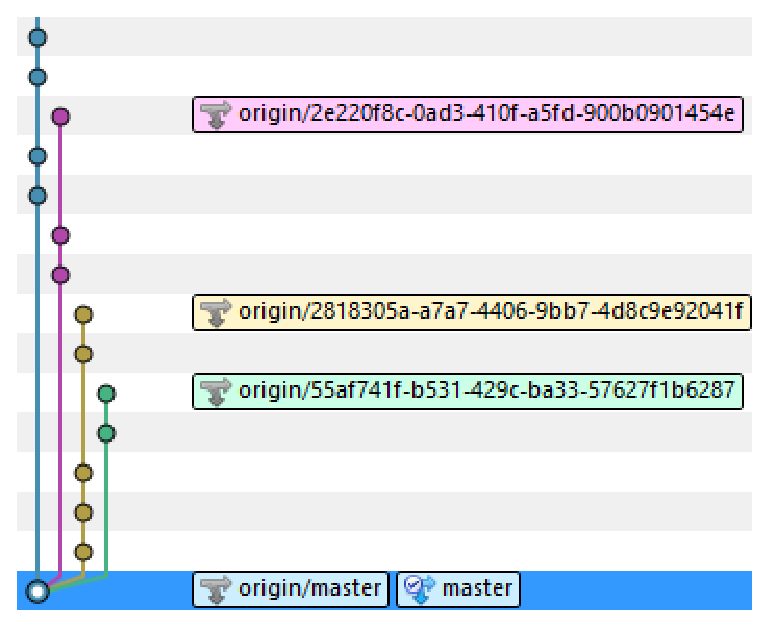
\includegraphics[scale=0.5]{images/tree.eps}
	\end{center}
\end{frame}

\begin{frame}[containsverbatim]
	\frametitle{Multi utilisateur}
	\begin{itemize}
	\item Chaque utilisateur a un numéro unique.
	\item Le champs lastUsed permet de charger la bonne session.
	\item Le tout formaté en JSON et sauvegardé dans un fichier dans \texttt{.plm}.
	\end{itemize}
	\begin{lstlisting}[language = plm,basicstyle={\tiny\ttfamily}, caption= plm.users]
[{"username":"Ced","lastUsed":true,"userUUID":"bed299bd-c446-4b06-b61d-6b5b9f310e64"}, {"username":"Viking","lastUsed":false,"userUUID":"9809cbb3-2264-4221-87a4-5d32d0a69d72"}, {"username":"Mat","lastUsed":false,"userUUID":"05cfd3d9-4a99-47f8-bec0-85e01f38d121"}]
	\end{lstlisting}
\end{frame}

\begin{frame}
	\frametitle{Serveur Play}
	\begin{center}
		
\begin{tikzpicture}[scale=0.65, every node/.style={scale=0.65}]
\node[server](PC1) at (-3,-1) {};
\node[xshift=-0.8cm,yshift=0.2cm,left of = PC1,align=left](PC1label) {Utilisateur A};

\node(GitA1) at (-5,-2.5) {\includegraphics[scale=0.25]{images/git.ps}}; 
\node[below of = GitA1,align=left](GitAlabel1) {Git local A1};

\node(GitA2) at (-2,-2.5) {\includegraphics[scale=0.25]{images/git.ps}}; 
\node[below of = GitA2,align=left](GitAlabel2) {Git local A2};

\node[server](PC2) at (3,-1) {};
\node[xshift=-0.8cm,yshift=0.2cm,left of = PC2,align=left](PC2label) {Utilisateur B};

\node(GitB) at (3,-2.5) {\includegraphics[scale=0.25]{images/git.ps}}; 
\node[xshift=-0.5cm,left of = GitB,align=left](GitBlabel) {Git local B};
\node[red,inner sep=0mm](croix) at (1.3,0.8) {\begin{LARGE}$\times$\end{LARGE}};

\node[server](PC3) at (4.5,0.5) {};
\node[xshift=0.6cm,right of = PC3,align=left](PC3label) {Utilisateur C};

\node(GitC) at (5.5,-0.5) {\includegraphics[scale=0.25]{images/git.ps}}; 
\node[xshift=0.7cm,right of = GitC,align=left](GitClabel) {Git local C};


\node[my cloud, minimum width=1.25cm, minimum height=1.55cm,font=\large] (cloud) at (0,2) {Internet};

\node(Git) at (-3.5,3) {\includegraphics[scale=0.5]{images/git.ps}}; 
\node[xshift=-1cm,left of = Git,align=left](Gitlabel) {Git central};

\node(Play) at (3.5,4) {
\includegraphics[scale=0.15]{images/play.eps}}; 
\node[above of = Play,align=left](Playlabel) {Serveur Play};

\node[server](PCprof) at (6.2,4) {};
\node[xshift=0.8cm,right of = PCprof,align=left](PCproflabel) {Poste professeur};

\draw[thick,darkgray!10!gray] (PC1.north west)--(cloud);
\draw[thick,darkgray!10!gray] (PC1.south east)--(GitA1);
\draw[thick,darkgray!10!gray] (PC1.south west)--(GitA2);
\draw[thick,darkgray!10!gray] (PC2.north east)--(1.3,0.8);
\draw[thick,darkgray!10!gray] (PC2.south)--(GitB);
\draw[thick,darkgray!10!gray] (PC3.north east)--(cloud);
\draw[thick,darkgray!10!gray] (PC3.south)--(GitC);
\draw[thick,darkgray!10!gray] (Git.east)--(cloud);
\draw[thick,darkgray!10!gray] (Play.south west)--(cloud);
\draw[thick,darkgray!10!gray] (Play.east)--(PCprof);
\path[->, red,line width = 0.5mm] (Git)  edge   [bend left=-20]   node {} (Play);
\path[<->, blue,line width = 0.5mm] (GitA2)  edge   [bend left=-80]   node {} (Git.east);
\path[->, darkgray!90,line width = 0.5mm] (PC3) edge [bend left=70] node{} (Play.south west);

\path[<->, blue,line width = 0.5mm] (-4.5,-5)  edge [auto]  node {Git push/pull} (-2,-5);
\path[->, red,line width = 0.5mm] (0,-5)  edge [auto]  node {Git pull} (2.5,-5);
\path[->, darkgray!90,line width = 0.5mm] (4.5,-5)  edge [auto]  node {Liaison d'identité} (7,-5);
\end{tikzpicture}

	\end{center}
\end{frame}

\begin{frame}
	\frametitle{Liaison d'identité}
	\begin{itemize}
	\item L'utilisateur peut lier sa véritable identité.
	\end{itemize}
	\begin{center}
		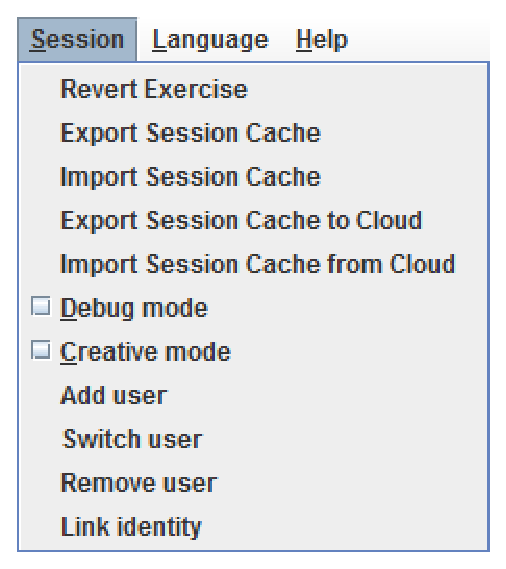
\includegraphics[scale=0.33]{images/menu.eps} $ \qquad$
		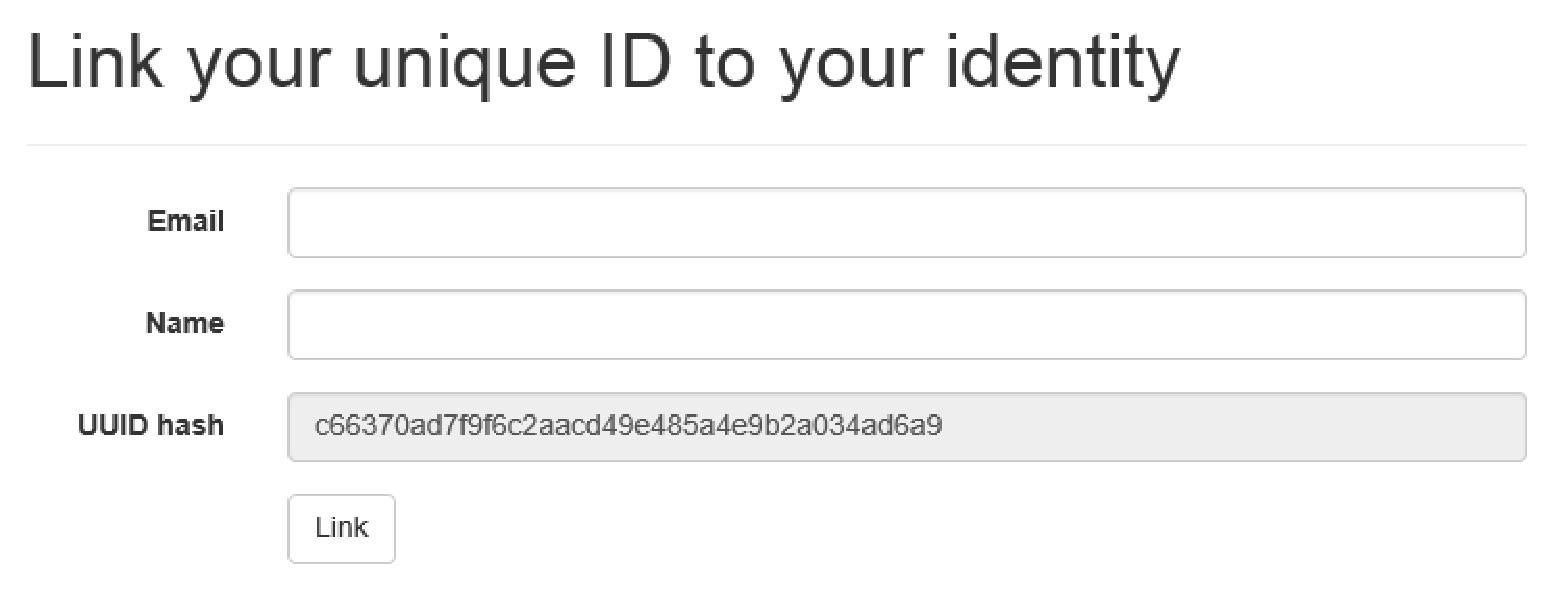
\includegraphics[scale=0.28]{images/link.eps}
	\end{center}
\end{frame}
\begin{frame}
	\frametitle{Liste des étudiants}
	\begin{itemize}
	\item Liste récapitulative des étudiants :
	\end{itemize}
	\begin{center}
		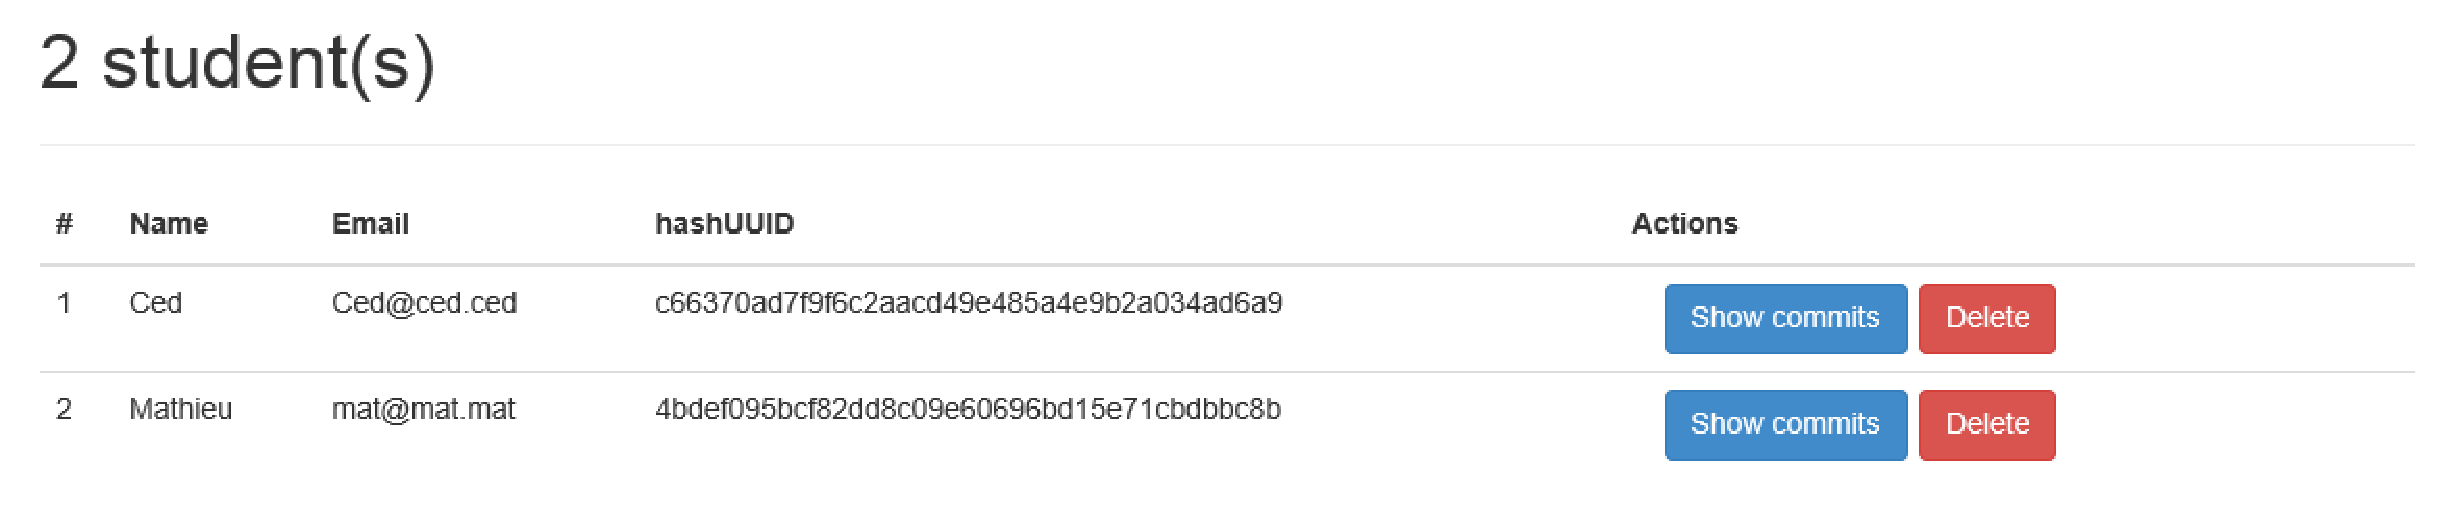
\includegraphics[scale=0.3]{images/students.eps}
	\end{center}
\end{frame}
\begin{frame}
	\frametitle{Récapitulatif d'un étudiant}
	\begin{center}
		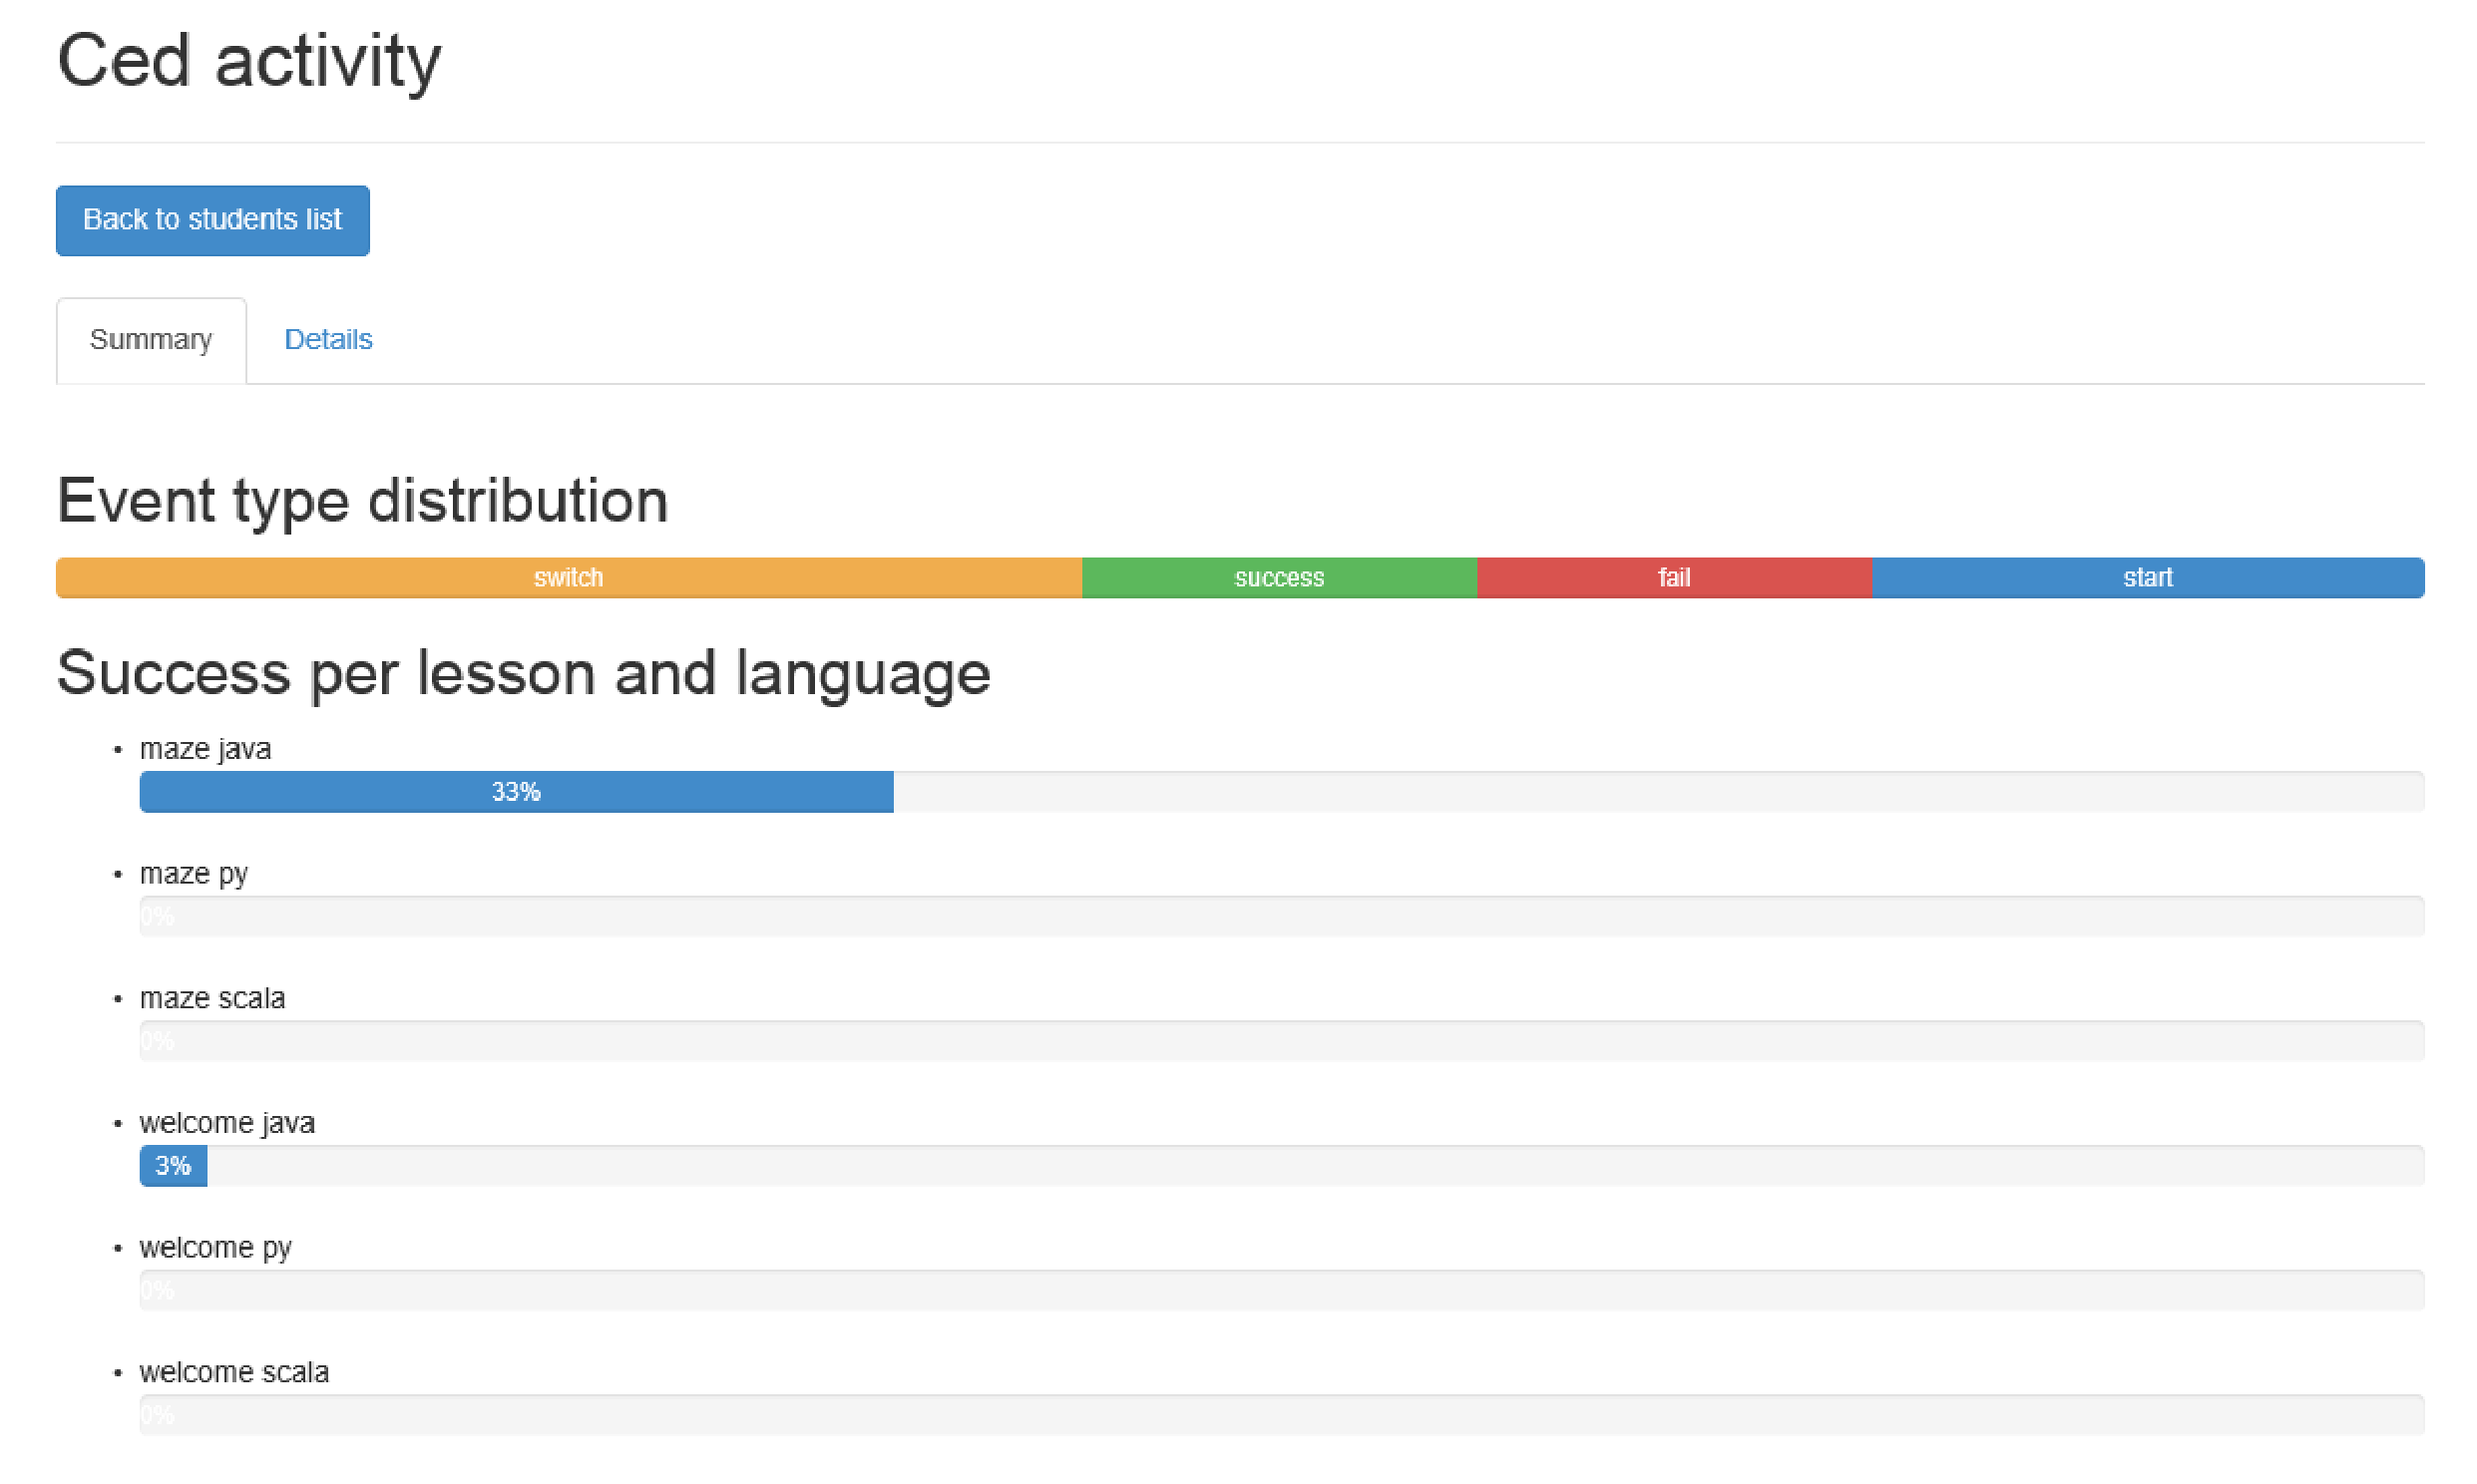
\includegraphics[scale=0.25]{images/summary.eps}
	\end{center}
\end{frame}
\begin{frame}
	\frametitle{Récapitulatif détaillé d'un étudiant}
	\begin{center}
		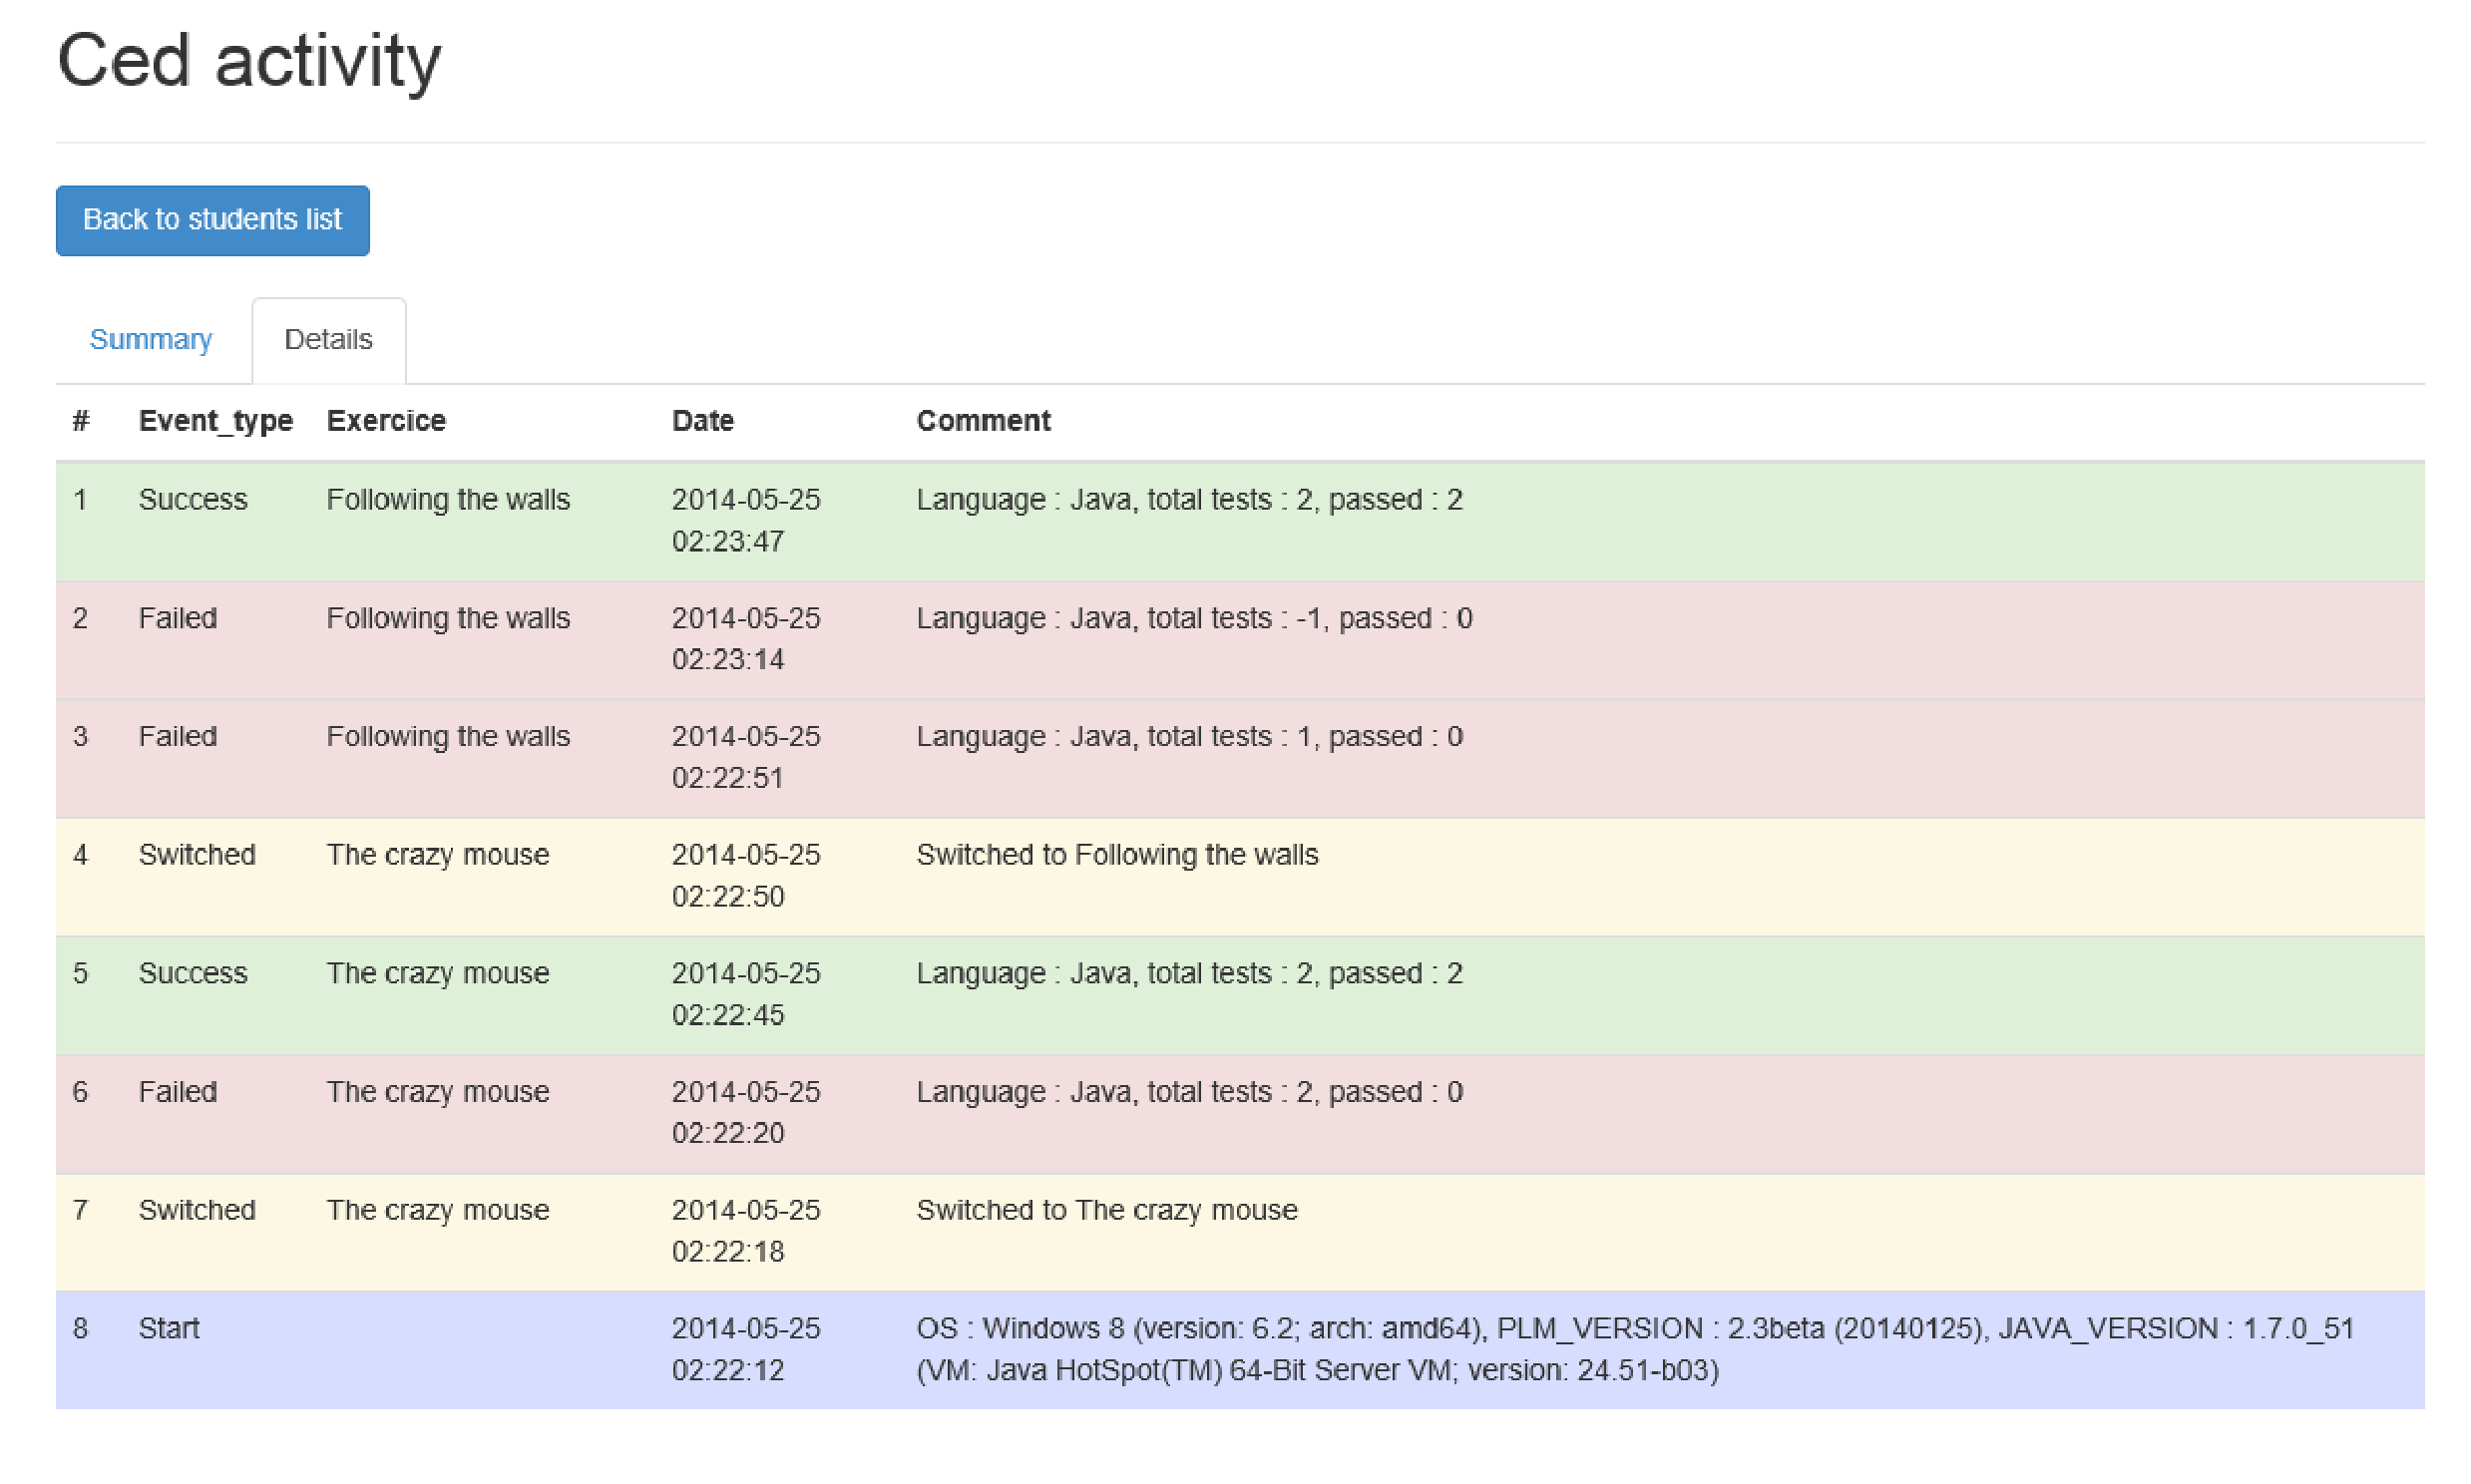
\includegraphics[scale=0.25]{images/details.eps}
	\end{center}
\end{frame}
\section{Conclusion}
	\begin{frame}
	\frametitle{Conclusion}
		\begin{itemize}
			\item PLM bien préparée à recevoir des modifications destinées aux professeurs ;
			\item Base stable pour évoluer ;
			\item Données collectées anonymes consultables publiquement ;
			\item Représentation graphique (\texttt{D3.js}).
		\end{itemize}
	\end{frame}	
\end{document}